%% 
%% Copyright 2007, 2008, 2009 Elsevier Ltd
%% 
%% This file is part of the 'Elsarticle Bundle'.
%% ---------------------------------------------
%% 
%% It may be distributed under the conditions of the LaTeX Project Public
%% License, either version 1.2 of this license or (at your option) any
%% later version.  The latest version of this license is in
%%    http://www.latex-project.org/lppl.txt
%% and version 1.2 or later is part of all distributions of LaTeX
%% version 1999/12/01 or later.
%% 
%% The list of all files belonging to the 'Elsarticle Bundle' is
%% given in the file `manifest.txt'.
%% 

%% Template article for Elsevier's document class `elsarticle'
%% with numbered style bibliographic references
%% SP 2008/03/01

\documentclass[preprint,12pt, a4paper]{elsarticle}

%% Use the option review to obtain double line spacing
%% \documentclass[authoryear,preprint,review,12pt]{elsarticle}

%% For including figures, graphicx.sty has been loaded in
%% elsarticle.cls. If you prefer to use the old commands
%% please give \usepackage{epsfig}

%% The amssymb package provides various useful mathematical symbols
\usepackage{amssymb}
%% The amsthm package provides extended theorem environments
%% \usepackage{amsthm}

%% The lineno packages adds line numbers. Start line numbering with
%% \begin{linenumbers}, end it with \end{linenumbers}. Or switch it on
%% for the whole article with \linenumbers.
\usepackage{lineno}
\usepackage{hyperref}
\usepackage{listings}

\lstset{ 
  language=R,                      % the language of the code
  basicstyle=\scriptsize\ttfamily, % the size of the fonts that are used for the code
  backgroundcolor=\color{white},   % choose the background color. You must add \usepackage{color}
  showspaces=false,                % show spaces adding particular underscores
  showstringspaces=false,          % underline spaces within strings
  showtabs=false,                  % show tabs within strings adding particular underscores
  frame=single,                    % adds a frame around the code
  rulecolor=\color{black},         % if not set, the frame-color may be changed on line-breaks within not-black text (e.g. commens (green here))
  tabsize=2,                       % sets default tabsize to 2 spaces
  captionpos=b,                    % sets the caption-position to bottom
  breaklines=true,                 % sets automatic line breaking
  breakatwhitespace=false,         % sets if automatic breaks should only happen at whitespace
  keywordstyle=\color{RoyalBlue},     % keyword style
  commentstyle=\color{YellowGreen},   % comment style
  stringstyle=\color{ForestGreen}     % string literal style
} 


\usepackage[usenames,dvipsnames]{color}    

\usepackage{float}
\restylefloat{table}

\journal{SoftwareX}

\begin{document}

\begin{frontmatter}

%% Title, authors and addresses

%% use the tnoteref command within \title for footnotes;
%% use the tnotetext command for theassociated footnote;
%% use the fnref command within \author or \address for footnotes;
%% use the fntext command for theassociated footnote;
%% use the corref command within \author for corresponding author footnotes;
%% use the cortext command for theassociated footnote;
%% use the ead command for the email address,
%% and the form \ead[url] for the home page:
%% \title{Title\tnoteref{label1}}
%% \tnotetext[label1]{}
%% \author{Name\corref{cor1}\fnref{label2}}
%% \ead{email address}
%% \ead[url]{home page}
%% \fntext[label2]{}
%% \cortext[cor1]{}
%% \address{Address\fnref{label3}}
%% \fntext[label3]{}

\title{pksensi: an R Package to Apply Global Sensitivity Analysis in
Physiologically Based Kinetic Modeling}

%% use optional labels to link authors explicitly to addresses:
%% \author[label1,label2]{}
%% \address[label1]{}
%% \address[label2]{}

\author[1]{Nan-Hung Hsieh}
\author[2]{Brad Reisfeld}
\author[1]{Weihsueh A. Chiu}

\address[1]{
Veterinary Integrative Biosciences, College of Veterinary Medicine and
Biomedical Sciences, Texas A\&M University, College Station, TX, USA\\
}
\address[2]{
Chemical and Biological Engineering and School of Biomedical
Engineering, Colorado State University, Fort Collins, CO, USA\\
}


\begin{abstract}
%% Text of abstract 
Sensitivity analysis (SA) is an essential tool for modelers to understand the influence of model parameters on model outputs. 
It is also increasingly used in developing and assessing pharmacokinetic models.
We developed an R package, named \textbf{pksensi}, to make global
sensitivity analysis more accessible in physiologically based
kinetic modeling. This package can investigate both parameter
uncertainty and sensitivity in pharmacokinetic models, including those
with multivariate model outputs, such as multiple time-points and tissue
compartments. We refined the extended Fourier Amplitude Sensitivity Test
method for SA by adding a random phase-shift to analyze the statistical
variability of the sensitivity index for each model parameter.
Furthermore, it includes functions to check the convergence of the
global SA results. Utilizing this package, we successfully
reproduced our previously published SA results of human physiologically
based pharmacokinetic modeling for acetaminophen and its two primary
metabolites. Overall, \textbf{pksensi} improves the user experience of
performing global SA and can create robust and reproducible results for
decision making in pharmacokinetic model calibration.

\end{abstract}

\begin{keyword}
%% keywords here, in the form: keyword \sep keyword
Global sensitivity analysis \sep  physiologically based kinetic modeling \sep Parameter fixing \sep R package

%% PACS codes here, in the form: \PACS code \sep code

%% MSC codes here, in the form: \MSC code \sep code
%% or \MSC[2008] code \sep code (2000 is the default)

\end{keyword}

\end{frontmatter}

\section*{Required Metadata}
\label{}

\section*{Current code version}
\label{}

Ancillary data table required for subversion of the codebase. Kindly replace examples in right column with the correct information about your current code, and leave the left column as it is.

\begin{table}[H]
\begin{tabular}{|l|p{6.5cm}|p{6.5cm}|}
\hline
\textbf{Nr.} & \textbf{Code metadata description} & \textbf{Please fill in this column} \\
\hline
C1 & Current code version & For example v42 \\
\hline
C2 & Permanent link to code/repository used for this code version & For example: $https://github.com/mozart/mozart2$ \\
\hline
C3 & Code Ocean compute capsule & For example: $https://codeocean.com/2017/07/30/neurospeech-colon-an-open-source-software-for-parkinson-apos-s-speech-analysis/code$\\
\hline
C4 & Legal Code License   & List one of the approved licenses \\
\hline
C5 & Code versioning system used & For example svn, git, mercurial, etc. put none if none \\
\hline
C6 & Software code languages, tools, and services used & For example C++, python, r, MPI, OpenCL, etc. \\
\hline
C7 & Compilation requirements, operating environments \& dependencies & \\
\hline
C8 & If available Link to developer documentation/manual & For example: $http://mozart.github.io/documentation/$ \\
\hline
C9 & Support email for questions & \\
\hline
\end{tabular}
\caption{Code metadata (mandatory)}
\label{} 
\end{table}


\linenumbers

%% main text

The permanent link to code/repository or the zip archive should include the following requirements: 

README.txt and LICENSE.txt.

Source code in a src/ directory, not the root of the repository.

Tag corresponding with the version of the software that is reviewed.

Documentation in the repository in a docs/ directory, and/or READMEs, as appropriate.




\section{Motivation and significance}
\label{}
Sensitivity analysis (SA) is a mathematical technique to investigate how
variations in model parameters affect model outputs. An increasing
number of studies use SA to determine which model parameters contribute
to high variation in model predictions \cite{ferretti2016trends}. This
technique has also been applied in pharmacology and toxicology research
\cite{loizou2015application, mcnally2012reconstruction}.
Pharmacokinetic (PK) models describe the changes in the concentrations
or amounts of a substance in the body over time (the various terms for
the kinetic models, including ``pharmacokinetic'', ``toxicokinetic'',
and ``biokinetic'' models, are used exchangeably here). The goal of SA
in PK research is to examine the sensitivity of output variables, such
as chemical concentration in blood or tissues, with respect to input
parameters, such as anatomical, physiological, and kinetic constants
\cite{mcnally2011workflow}. In addition, this SA approach can guide
experimental design and the parameter estimation processes
\cite{zhang2015sobol}. For instance, SA can identify ``unidentifiable''
parameters that can lead to problems with numerical procedures used in
parameter estimation \cite{chu2010quantitative}. It can be further
applied to parameter prioritization and parameter fixing before model
calibration \cite{fphar201800588}.

In our earlier work \cite{fphar201800588}, we developed an updated
workflow to apply global SA to reduce the computational burden in the
Bayesian, Markov Chain Monte Carlo (MCMC)-based calibration process of a
physiologically based pharmacokinetic (PBPK) model. We used GNU MCSim
\cite{bois2009gnu}, an effective simulation package for Bayesian
population PBPK modeling, to calibrate the model. We found that the
extended Fourier Amplitude Sensitivity Test (eFAST), a type of
variance-based global SA algorithm, had the best balance of efficiency
and accuracy for a sophisticated, multi-compartment, multi-dataset, and
multi-metabolite PBPK model. This method was first introduced in 1973, 
\cite{cukier1973study} in a study of the sensitivity of coupled reaction systems
that are constructed by differential equations with the numerous rate
coefficients (the classic FAST method with the first-order
effect only). It then evolved to estimate the Sobol' sensitivity measure
(the eFAST method with first- and
total-order effects) \cite{saltelli1999quantitative}. The FAST algorithm creates the multidimensional
space of input parameters through a ``search-curve''. It is more
computationally efficient in calculating the influence of model
parameter than other global SA methods such as the Monte Carlo based
approaches \cite{jansen1999analysis, owen2013better}. Our previous work
also found some efficient visualization approaches that can be used to
distinguish between ``influential'' and ``non-influential'' parameters.
This approach addresses common identifiability issues of PBPK model
parameter that increase the computational burden of Bayesian analysis
\cite{garcia2015identifiability}, and therefore reduce the
computational efficiency. We also developed approaches for communicating
parameter sensitivity in decision making.

There are numerous developed packages, such as sensitivity
\cite{R-sensitivity}, which is a practical tool to conduct local and
global SA. The sensitivity package includes some functions to
generate the parameter sequences by using different computing
algorithms. Also, it provides a feasible way to integrate external
modeling results. This computational approach can effectively solve the
heavy computing burden of numerical solutions within the pure R
environment. Several other R packages, such as FME,
multisensi, and ODEsensitivity include SA tools and
are freely available in the Comprehensive R Archive Network (CRAN). The
FME package contains a basic method for performing local SA
for dynamic models \cite{JSSv033i03}. It can also conduct collinearity
and identifiability analysis to evaluate which model parameters can
estimate or exclude based on available observation data. The
multisensi package provides SA for models with multivariate
output \cite{R-multisensi}. ODEsensitivity can perform SA in
ordinary differential equation (ODE) models \cite{R-ODEsensitivity}. It
utilizes the ODE interface from the deSolve package and
connect it with the SA from the sensitivity package. Other
related packages such as mtk \cite{RJ-2015-031} and
fast \cite{R-fast} are designed to investigate the importance
of model parameter.

Although these tools provide various approaches to perform SA, they each
individually have limitations for application to PK modeling. For
example, the estimated index in SA is not robust when using the
inadequate size of the sample number. However, there are no software
packages that provide the available tools in the assessment of
reliability. In addition, the existing eFAST function does not include
the feature to generate the random sampling curve. We present here an
package, called \textbf{pksensi}, which is designed to make SA more
accessible and reproducible in pharmacological and toxicological
researches. 

\section{Software description}
\label{}

Our package can investigate both parameter uncertainty and
sensitivity in PK model with multivariate model outputs. Moreover, it
seamlessly integrates with both general ODE solvers available in R or as
external C code, as well as the GNU MCSim software used for conducting
sophisticated PK modeling, including MCMC. The analytical framework in
\textbf{pksensi} includes not only global SA but also the uncertainty
analysis and diagnostic tools to support the modeling process.

\subsection{Installation}
\label{installation}

This package can link with R deSolve package,
which includes a comprehensive integrator to solve ODE. The GNU MCSim
can be installed by following the instruction in GNU MCSim's manual on
\url{https://www.gnu.org/software/mcsim/mcsim.html} or using the
built-in \textbf{\textit{mcsim\_install()}} function in \textbf{pksensi}.

\subsection{Parameter matrix generation}
\label{parameter-matrix-generation}

We adopted eFAST, the widely used analysis of variance (ANOVA)-like
global SA approach to decompose the variance to partial variances for
multidimensional parameters in numerical models in this package. Most of
the available eFAST functions, such as the algorithm to generate the
parameter space and to set the sampling frequency, were sourced from the
R sensitivity package \cite{R-sensitivity}. The eFAST method
computes the sensitivity index (SI) via ANOVA-like decomposition of the
function for analysis. This type of global SA approach and SI also know
as Sobol' method and Sobol' index. Since the estimated SI is not stable
(high variation) when using smaller sample size, we included a random
phase-shift approach to conduct replicating sampling from random
starting points across parameter space to test the convergence and
robustness of the sensitivity measurement. Considering the model that is
built under \(y=f(x_{i})\). The sampling scheme can describe as,

\[ x_i = \frac{1}{2} + \frac{1}{\pi}\arcsin(\sin(\omega_is + \varphi_i)) \]


where \(x_i\) is the nominal value of the \(i\)-th parameter, and
\(\omega_i\) is a vector giving the set of frequencies, one frequency
for each parameter, and \(\varphi\) is a random phase-shift coefficient
ranged from 0 to \(2\pi\). Through the random
phase-shift, the robust result of the sensitivity measurement should be
similar across each replication under the same sample size. For most
Sobol'-based SA algorithms, the larger sample size is needed to reduce
the probability of having negative estimates. However, FAST estimates
are always positive according to its construction.

To investigate the convergence of SI, we adopted the ``exam'' approach that
proposed previously \cite{sarrazin2016global}. This method quantitatively
assesses convergence by computing the width of 95\% confidence intervals
of computed SI for all parameters across all time-points and output
variables. Through random phase-shift procedure, the replicated SI
values can repeatedly sample independently. Therefore, they can be used
to investigate the convergence of SI as,

\[CI_{i,t} = max(SI_{i,t}^{ub}-SI_{i,t}^{lb})\]

where \(SI_{i,t}^{ub}\) and \(SI_{i,t}^{ub}\) are the upper and lower
bound of the SI from the specific model output (\(i\)) at time (\(t\)).
\(CI_{i,t}\) is the corresponding convergence index.

To integrate the random phase-shift with eFAST, we built the
\textbf{\textit{rfast99()}} function, which can be used to perform the sensitivity
test for the whole modeling process. The function can sample and generate the testing parameter matrix
based on a given argument of sample size \(n\) and probability
distribution (e.g., mean/s.d. of normal distribution, meanlog/sdlog of
log-normal distribution, and minimum/maximum of uniform distribution).
The number of model evaluations is equal to the sample size times the
number of model parameters.

\subsection{Modeling}\label{modeling}

The \textbf{pksensi} provides a useful function to solve ODEs
in PK models using analytical and numerical approaches. The solution can
perform under the pure R programming environment by linking
with R deSolve package \cite{JSSv033i09}.
However, the most efficient way to achieve high computational speed is
through compiled, lower-level languages, such as FORTRAN, C, or C++. 
Therefore, it includes a function to compile and create
dynamic-link libraries (.dll) on Windows and shared objects (.so) on
Unix-liked systems (e.g., Linux and MacOS). This compiled program can
load and execute through the build-in function in R. However, Windows
users need to install Rtools to compile the source code by using the GNU
GCC compiler. The C implementation of the example model can be found as
an example within GNU MCSim \cite{bois2009gnu}. The \textbf{pksensi}
can also link with GNU MCSim to create the model program, used in
solving each system of equations.

The uncertainty analysis is a crucial modeling process within SA.
Sometimes, it is difficult to have informative data to set up the
parameter distribution. A wider range for a parameter distribution might
cause a numerical error at extreme values. On the other hand, narrower
ranges might cause the incorrect calibrated result of the model
parameter. The uncertainty analysis using Monte Carlo is an appropriate
approach in the data-driven modeling process to address this problem.
Before fitting the data to model, the Monte Carlo can be applied with
the given distribution of model parameter to examine whether the
experimental data are within the range of the distribution of model
output. The \textbf{pksensi} also has a function that can link to GNU MCSim
to conduct Monte Carlo analysis, which is built-into GNU MCSim and
examine the simulation result. The general workflow of uncertainty and
SA is illustrated in Figure \ref{fig:workflow}.

\begin{figure}
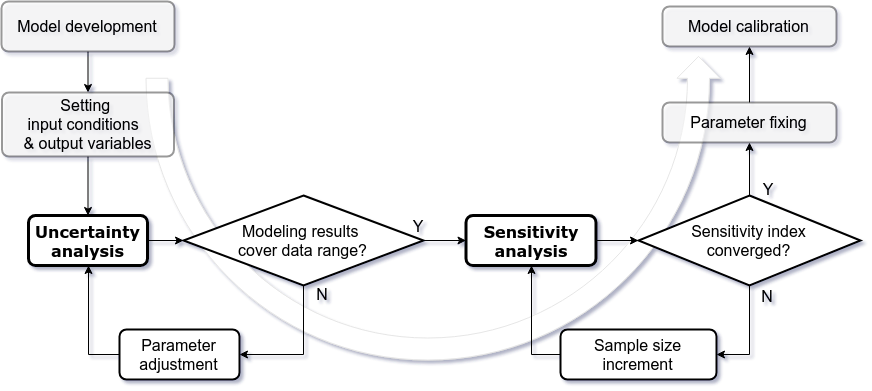
\includegraphics[width=1\linewidth]{workflow} \caption{\label{fig:workflow}Workflow for performing uncertainty and sensitivity analysis.}\label{fig:workflow}
\end{figure}

\subsection{Output visualization and decision
support}\label{output-visualization-and-decision-support}

The output of SA returns a list that contains the given time-points and
values of all state variables (e.g., chemical concentrations in blood and other tissues).
This format is particularly suited for further graphical routines within
\textbf{pksensi}. Also, time-dependent sensitivity measurements of
first and total effects for all parameters can be plotted
simultaneously. If the computed SI show different values across
replications under the same sample size, this indicates an inadequate
sample number, which can create an unreliable result. It is essential to
use a sufficient sample size to prevent incorrect judgments in parameter
fixing. The package includes functions to check the convergence
and sensitivity of model parameters, providing a means to assess the
robustness of the sensitivity measurement. We also developed a
``cut-off''-based approach in this package to distinguish between
``influential'' and ``non-influential'' parameters. Finally,
this package also provides visualization tools for the effective
investigation and communication of results in decision support.

\section{Illustrative Examples}
\label{}

Two PK models will apply to demonstrate how
\textbf{pksensi} works. The first one is a generic model, and the
second is a chemical-specific model.

\subsection{Equations}
\label{equations}

In the first example, we use a generic, one-compartment PK model from
httk package \cite{JSSv079i04} to demonstrate how
\textbf{pksensi} can apply to PK studies. The differential equations
for this model is as,

\[\frac{dA_{gutlumen}}{dt} = -k_{gutabs} \cdot A_{gutlumen} + g(t)\]
\[\frac{dA_{rest}}{dt} = k_{gutabs} \cdot A_{gutlumen}-k_{elim} \cdot A_{rest}\]

where \(A_{gutlumen}\) is the state variable that describes the quantity
of compound in the gut lumen (mg) and \(A_{rest}\) is the quantity of
compound in rest of body and blood (mg). The parameter \(k_{gutabs}\) is
the absorption rate constant that describes the chemical absorption from
the gut lumen into gut tissue through first-order processes (/h) and
\(k_{elim}\) is the elimination rate constant (/h), which is equal to
the total clearance divided by the volume of distribution. The
time-dependent function \(g(t)\) is used to describe the oral dosing
schedule.

The concentration of the chemical in the rest of body and blood
(\(C_{rest}\), mg/L) can calculate as,

\[ C_{rest} = A_{rest} / V_{dist} \cdot BW\]

where \(V_{dist}\) is the volume of distribution (L/kg BW) and \(BW\) is
the body weight (kg). \(C_{rest}\) can also represent as the chemical
concentration in plasma that can be further used to compare with
observed results in a PK experiment. The bioavailability is assumed to
be 100\% in this model.

To start, we implemented the one-compartment PK model in R. The
\textbf{pksensi} allows users select the preferred method to solve the
PK model, either with the deSolve package or with GNU MCSim
through the compile function. This section mainly focuses on how to
conduct global SA with deSolve package with pure R
environment.


The one-compartment PK model can describe the quantity of compound in
the gut lumen (\(Agutlument\)) and the rest of body
(\(Agutlument\).) The \(Ametabolized\) is the quantity of
compound transform and metabolize through hepatic clearance.

\begin{lstlisting}
pbtk1cpt <- function(t, state, parameters) {
  with(as.list(c(state, parameters)), {
    dAgutlument = - kgutabs * Agutlument
    dAcompartment = kgutabs * Agutlument - ke * Acompartment
    dAmetabolized = ke * Acompartment
    Ccompartment = Acompartment / vdist * BW;
    list(c(dAgutlument, dAcompartment, dAmetabolized), 
         "Ccompartment" = Ccompartment) 
  })
}
\end{lstlisting}

The parameter values and initial states need to be assigned to specific
values before simulation. Here, we use the corresponding parameter value
of acetaminophen (APAP) in this example. These model parameters are
derived from the \emph{in-vivo} or \emph{in-vitro} experiment results.
The parameter value can be generated from \(parameterize\_1comp\)
function in httk package as:

\begin{lstlisting}
library(httk)
pars1comp <- (parameterize_1comp(chem.name = "acetaminophen"))
initState <- c(Agutlument = 10, Acompartment = 0, Ametabolized = 0)
\end{lstlisting}

The given value of \(vdist\), \(ke\), and \(kgutabs\) in httk are 1.1 (L/kg BW), 0.23 (/h), and 2.18 (/h),
respectively. The body weight is assumed to be 70 (kg). 
In addition, the initial state condition (\(initState\)) need to specify in model solving.







\section{Impact}
\label{}

We initiated \textbf{pksensi} in order to facilitate a comprehensive
and efficient global SA workflow in PK modeling, filling a crucial gap
for open-source modeling communities. It provides a straightforward
application to investigate the impact of parameters on model outputs
across simulation time-points and variables. We adopted the eFAST
method, a common variance-based SA that we found to have the best
balance of efficiency and accuracy. In addition, the package also
includes the ability to assess the convergence of SA results, which is
rarely addressed in most global SA studies and software packages. We
also developed functions to visualize the output results and help
distinguish the ``influential'' and ``non-influential'' parameters that
can be applied in parameter fixing in the model calibration. 

We chose to integrate sensitivity analysis with GNU MCSim because it is
a powerful open-source software package for dynamical simulation of
biological-based models, mainly built for PK research with probabilistic
approaches \cite{bois2009gnu}. In addition, the current version of
\textbf{pksensi} includes both GNU MCSim and deSolve package as the
main ODE solvers. Compared with the deSolve package, the GNU
MCSim can provide better speed and efficiency to solve the ODEs in PK
models. Although \textbf{pksensi} provides the essential features and
functions to install and link with GNU MCSim, conducting the uncertainty
and SA in PK modeling, the overall learning curve of this workflow might
steep for users that are not familiar with GNU MCSim from model
development, debugging, and testing. Therefore, the general package,
such as deSolve, can be an alternative option for R users. It addition,
\textbf{pksensi} also has potential to be performed in interactive PBPK
modeling platform that was mentioned in rencent study \cite{li2019integration}.

\section{Conclusions}
\label{}

Overall, \textbf{pksensi} provides comprehensive suite of features and
functions for performing global SA for PK models and can create robust
and reproducible results for decision making in model development and
calibration. Although \textbf{pksensi} used here is mainly for PK
modeling, it can also be applied to other ODE-based dynamic models in
order to investigate the sensitivity of model outputs to input
parameters.

\section{Conflict of Interest}

We wish to confirm that there are no known conflicts of interest associated with this publication and there has been no significant financial support for this work that could have influenced its outcome.

\section*{Acknowledgements}
\label{}

This work was funded, in part, by grant 1U01FD005838 from the U.S. Food
and Drug Administration (FDA) and grant P42 ES027704 from the U.S.
National Institute of Environmental Health Sciences. This article
reflects the views of the author and should not be construed to
represent FDA's views or policies. We thank Dr.~Yasha Hartberg and
Dr.~Barbara Gastel at the Texas A\&M University, Dr.~Frederic Bois from
Certara and Dr.~Eleftheria Tsakalozou from U.S. FDA for reviewing the
manuscript and consultation.

%% The Appendices part is started with the command \appendix;
%% appendix sections are then done as normal sections
%% \appendix

%% \section{}
%% \label{}

%% References:
%% If you have bibdatabase file and want bibtex to generate the
%% bibitems, please use
%%
%%  \bibliographystyle{elsarticle-num} 
%%  \bibliography{<your bibdatabase>}

%% else use the following coding to input the bibitems directly in the
%% TeX file.



\bibliographystyle{elsarticle-num} 
\bibliography{j.softx.pksensi}


\section*{Current executable software version}
\label{}

Ancillary data table required for sub version of the executable software: (x.1, x.2 etc.) kindly replace examples in right column with the correct information about your executables, and leave the left column as it is.

\begin{table}[!h]
\begin{tabular}{|l|p{6.5cm}|p{6.5cm}|}
\hline
\textbf{Nr.} & \textbf{(Executable) software metadata description} & \textbf{Please fill in this column} \\
\hline
S1 & Current software version & For example 1.1, 2.4 etc. \\
\hline
S2 & Permanent link to executables of this version  & For example: $https://github.com/combogenomics/$ $DuctApe/releases/tag/DuctApe-0.16.4$ \\
\hline
S3 & Legal Software License & List one of the approved licenses \\
\hline
S4 & Computing platforms/Operating Systems & For example Android, BSD, iOS, Linux, OS X, Microsoft Windows, Unix-like , IBM z/OS, distributed/web based etc. \\
\hline
S5 & Installation requirements \& dependencies & \\
\hline
S6 & If available, link to user manual - if formally published include a reference to the publication in the reference list & For example: $http://mozart.github.io/documentation/$ \\
\hline
S7 & Support email for questions & \\
\hline
\end{tabular}
\caption{Software metadata (optional)}
\label{} 
\end{table}

\end{document}
\endinput
%%
%% End of file `SoftwareX_article_template.tex'.
